\chapter{Background}
\label{Chapter2}
In this chapter, we provide some background notions about the main concepts related to the thesis work. In particular, more details are given with regard to the two principal components of the proposed model (i.e., \textit{Random And Tensorized SPNs} and \textit{abduction}) and the faced classification task.

\section{Neural-Symbolic integration}
The goals of neural-symbolic computation are to provide a coherent, unifying view for logic and connectionism\footnote{\textit{Connectionism} is an approach in the fields of cognitive science that hopes to explain mental phenomena using artifical neural networks.}, to contribute to the modelling and understanding of cognition and, thereby, behaviour, and to produce better computational tools for integrated machine learning and reasoning. To this end, logic and network models are studied together as integrated models of computation. Typically, translation algorithms from a symbolic to a connectionist representation and vice-versa are employed to provide either (\textit{i}) a neural implementation of a logic, (\textit{ii}) a logical characterisation of a neural system, or (\textit{ii}) a hybrid learning system that brings together features from connectionism and symbolic artificial intelligence.

From a theoretical perspective, these efforts appear well-founded. According to our current knowledge and understanding, both symbolic/cognitive and sub-symbolic/neural models—especially when focusing on physically-realisable and implementable systems (i.e. physical finite state machines) rather than strictly abstract models of computation, together with the resulting physical and conceptual limitations—seem formally equivalent in a very basic sense: notwithstanding partially differing theoretical arguments, both paradigms are considered in practice equivalent concerning computability \cite{10.5555/343643}. Also from a tractability perspective, for instance in \cite{Rooij2008099398432}, equivalence in practice with respect to classical dimensions of analysis (i.e. interchangeability except for a polynomial overhead) has been established. Finally, \cite{Leitgeb200508189202146} provided an \textit{in principle} existence result, showing that there is no substantial difference in representational or problem-solving power between dynamical systems with distributed representations and symbolic systems with non-monotonic reasoning capabilities.

But while these findings provide a solid foundation for attempts at closing the gap between connectionism and logic, many questions nonetheless remain unanswered especially when crossing over from the realm of theoretical research to implementation and application, among others switching from compositional symbols denoting an idealised reality to virtually real-valued vectors obtained from sensors in the real world: although introducing basic connections and mutual dependencies between the symbolic and the subsymbolic paradigm, the levels of analysis are quite coarse and almost all results are only existential in character. For instance, while establishing the in principle equivalence described above, \cite{Leitgeb200508189202146} does not provide constructive methods for how to actually obtain the corresponding symbolic counterpart to a sub-symbolic model and vice versa.

Still, over the last decades several attempts have been made at developing a general neural-symbolic framework, usually trying to apply the most popular methods of their respective time—such as currently modular deep networks. Growing attention has been given recently to deep networks where it is hoped that high-level abstract representations will emerge from low-level unprocessed data \cite{10.1162/neco.2006.18.7.1527}. Most modern neural-symbolic systems use feedforward and recurrent networks, but seminal work in the area used symmetric networks \cite{Pinkas1991062822913} of the kind applied in deep learning, and recent work starts to address real applications of symmetric neural-symbolic networks \cite{dePenning201001}. There, in general each level of a neural-symbolic system represents the knowledge evolution of multiple agents over time. Each agent is represented by a network in this level encoding commonsense (nonmonotonic) knowledge and preferences. The networks/agents at different levels can be combined upwards to represent relational knowledge and downwards to create specialisations, following what is known as a network-fibring methodology \cite{10.5555/1597148.1597205}. Fibring is just one example of how principles from symbolic computation (in this case, recursion) can be used by connectionism to advance the research in this area.

One of the most relevant example of neural-symbolic integration is DeepProbLog \cite{10.5555/3327144.3327291}, a probabilistc logic programming language that incorporates deep learning by means of neural predicates. It supports (\textit{i}) both symbolic and sub-symbolic representations and inference, (\textit{ii}) program induction, (\textit{iii}) probabilistic (logic) programming and (\textit{iv}) (deep) learning from examples. The relevance of this work lies in the fact that it is the first to propose a framework where general-purpose neural networks and expressive probabilistic-logical modeling and reasoning are integrated in a way that exploits the full expressiveness and strengths of both worlds and can be trained end-to-end based on examples.

\section{Sum-Product Networks (SPNs)}
Sum-Product Networks (SPNs) were proposed by Poon and Domingos \cite{poon2011sum} in 2011 as a modification of Darwiche's \cite{Darwiche:2002fj}, \cite{DBLP:journals/corr/abs-1301-3847} arithmetic circuits. Every SPN consists of a directed graph that represents a probability distribution resulting from a hierarchy of distributions combined in the form of mixtures (sum nodes) and factorizations (product nodes), as shown in Figure \ref{fig:spn}. SPNs, like arithmetic circuits, can be built by transforming a probabilistic graphic model \cite{koller2009probabilistic}, such as Bayesian network or a Markov Network, but they can also be learned from data. The main advantage of SPNs is that several inference tasks can be performed in time proportional to the number of links in the graph.

More formally:

\begin{definition}{\textbf{(Sum-Product Network - SPN)}}
\label{def:evi}
An SPN $C$ consists of a rooted acyclic directed graph such that:
\begin{enumerate}[I.]
  \item every leaf node represents a univariate probability distribution;
  \item all the other nodes are either of type sum or product;
  \item all the parents of a sum node (if any) are product nodes, and vice versa;
  \item $n_i \rightarrow n_j$ outgoing from a sum node has an associated weight, $w_{ij} \geq 0$.
\end{enumerate}
\end{definition}

\begin{figure}[H]
\caption{Two examples of SPNs.}
\label{fig:spn}
\centering
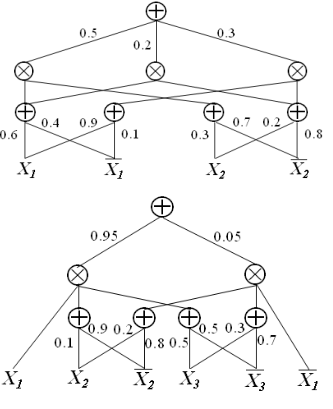
\includegraphics[scale=0.6]{Figures/SPN.png}
\end{figure}
The probability distribution of each leaf node is defined on a variable $V$, which can have finite states or be continuous. In the first case, the distribution is usually degenerate, i.e., there is a particular value $v^{*}$ of $V$ such that $P(v^{*}) = 1$ and $P(v) = 0$ otherwise (\textit{indicator}). When $V$ is continuous, the probability distribution can be Gaussian \cite{pmlr-v28-gens13}, \cite{pmlr-v32-rooshenas14}, piecewise polynomial \cite{DBLP:journals/corr/abs-1710-03297}, etc. (SPNs can be further generalized by allowing each terminal node to represent a multivariate probability density - for example, a multivariate Gaussian \cite{DBLP:journals/corr/DesanaS16} or a Chow-Liu tree \cite{10.1007/978-3-319-23525-7_21}).

An SPN can be built bottom-up beginning with sub-SPNs of one node and joining them with sum and product nodes. All the definitions of SPNs can be established recursively, first for one-node SPNs, and then for sum and product nodes. Similarly, all the properties of SPNs can be proved by structural induction.

If the probability distribution of a leaf node is defined on $V$, its \textit{scope} is the set ${V}$. If $n_i$ is a sum or a product node, its \textit{scope} is the union of the scopes of its children. Let $\mathsf{ch(n)}$ denote the set of children of a node. The \textit{scope} of an SPN, denoted by $\phi(\mathsf{S})$, is the scope of its root, $\phi(\mathsf{n_r})$. The variables in the scope of an SPN are sometimes called \textit{model variables} (in contrast with \textit{latent variables}.

Without going into detail, SPNs parameter learning consists in finding the optimal parameters for an SPN given its graph and a dataset. In generative learning the most common optimality criterion is to maximize the likelihood of the parameters of the model given a dataset, while in discriminative learning the goal is to maximize the conditional likelihood for each value of a variable C, called the class.

SPN allow to perform \textit{probabilistic inference}, i.e. deriving the probability of one or more RVs taking a specific value or a set of values. Exact and efficient probabilistic inference is important when we want to reason and quickly take complex decisions in presence of uncertainty in real-world scenarios. Probabilistic inference can be organized in classes of queries. Informally, a class of queries comprises of all the queries that share the same "structure", and hence present the same computational challenges. More formally, a class of queries is a collection of functions that operate on probability distributions and that can be characterized by the mean of their inputs, outputs and/or by the operations their computation involves \cite{ProbCirc20}. Here, we report several classes of queries which are used to compare and classify probabilistc models. 

\begin{definition}{\textbf{(Complete evidence queries - $\mathsf{EVI}$)}}
\label{def:evi}
The class of complete evidence queries $\boldsymbol{\mathcal{Q}}_{\mathsf{EVI}}$ is the set of queries that compute the probability $p_{\mathbf{X}}(\mathbf{x})$ for any complete evidence $\mathbf{x} \in \mathsf{val}(\mathbf{X})$.
\end{definition}

\begin{definition}{\textbf{(Marginal queries - $\mathsf{MAR}$)}}
\label{def:mar}
The class of marginal queries $\boldsymbol{\mathcal{Q}}_{\mathsf{MAR}}$ is the set of queries that compute the probability $p_{\mathbf{X}}(\mathbf{y})$ for any partial evidence $\mathbf{y} \in \mathsf{val}(\mathbf{Y})$, where $\mathbf{Y} \subseteq \mathbf{X}$.
\end{definition}

\begin{definition}{\textbf{(Conditional queries - $\mathsf{CON}$)}}
\label{def:con}
The class of conditional queries $\boldsymbol{\mathcal{Q}}_{\mathsf{CON}}$ is the set of queries that compute the probability $p_{\mathbf{X}}(\mathbf{y} | \mathbf{z})$ for any $\mathbf{y} \in \mathsf{val}(\mathbf{Y})$ and $\mathbf{z} \in \mathsf{val}(\mathbf{Z})$ , where $\mathbf{Y} \cup \mathbf{Z} = \mathbf{X}$ and $\mathbf{Y} \cap \mathbf{Z} = \varnothing$.
\end{definition}
It should be noticed that is possible to easily define the class $\boldsymbol{\mathcal{Q}}_{\mathsf{CON}}$ in terms of $\boldsymbol{\mathcal{Q}}_{\mathsf{EVI}}$ and $\boldsymbol{\mathcal{Q}}_{\mathsf{MAR}}$ by noting that any conditional query $p(x|y)$ can be rewritten as $p(x,y) / p(y)$.

\begin{definition}{\textbf{(Maximum a posteriori queries - $\mathsf{MAP}$)}}
\label{def:map}
The class of maximum a posteriori queries $\boldsymbol{\mathcal{Q}}_{\mathsf{MAP}}$ is the set of queries that compute:
\begin{align*}
	\argmax_{z \in \mathsf{val}(\mathbf{Z})} p_{\mathbf{X}}(\mathbf{z}|\mathbf{y}) = \argmax_{z \in \mathsf{val}(\mathbf{Z})} p_{\mathbf{X}}(\mathbf{z},\mathbf{y})
\end{align*}
where $\mathbf{Y} \cup \mathbf{Z} = \mathbf{X}$ and $\mathbf{Y} \cap \mathbf{Z} = \varnothing$.
\end{definition}
More classes of queries can be defined by "combining" the previous ones.
This is the case for marginal $\mathsf{MAP}$ queries ($\boldsymbol{\mathcal{Q}}_{\mathsf{MMAP}}$), involving marginalization over one subset of RVs and maximization over another one.

Recently, new advanced probabilistic queries have been introduced in literature.
These  include  computing  the  probability  of  an  event  described  as  a  complex logical sentence (e.g., involving disjunctions) \cite{choi2015tractable}; computing expectations of probabilistic predictive models \cite{khosravi2019tractable} and information theoretic quantities of a distribution such as its entropy or the Kullback-Leibler divergence between distributions \cite{liang2017towards}.
In the following, we will refer to the class of advanced queries as $\boldsymbol{\mathcal{Q}}_{\mathsf{ADV}}$.

Several well-known structural properties allow us to categorize PCs w.r.t. the classes of queries they make tractable.
% In fact, to make a class of queries $\boldsymbol{\mathcal{Q}}$ tractable for a PC, this has to satisfy specific structural constraints.
In the following, we first report the definition of tractability and then such structural properties indicating the class of queries they make tractable if satisfied.

\begin{definition}{\textbf{(Tractability)}}
A class of queries $\boldsymbol{\mathcal{Q}}$ is tractable on a family of probabilistic models $\mathcal{M}$ iff any query $q \in \boldsymbol{\mathcal{Q}}$ on a model $\mathsf{m} \in \mathcal{M}$ can be computed in time $O(poly(|\mathsf{m}|))$, where $|\mathsf{m}|$ is the size of the model.
\end{definition}

\begin{definition}{\textbf{(Smoothness, \textit{aka} Completeness)}}
A probabilistic circuit is \textbf{\textit{smooth}} if for each sum node $\mathsf{S}$ it hols that:
\begin{equation}\label{eq:completeness}
\forall \mathsf{C_1},\mathsf{C_2} \in \mathsf{ch}(\mathsf{S}) : \phi(\mathsf{C_1}) = \phi(\mathsf{C_2})
\end{equation}
\end{definition}

\begin{definition}{\textbf{(Decomposability)}}
A probabilistic circuit is \textbf{\textit{decomposable}} if for each product node $\mathsf{P}$ it hols that:
\begin{equation}\label{eq:decomposability}
\forall \mathsf{C_1},\mathsf{C_2} \in \mathsf{ch}(\mathsf{P}), \mathsf{C_1} \neq \mathsf{C_2} : \phi(\mathsf{C_1}) \cap \phi(\mathsf{C_2}) = \varnothing
\end{equation}
\end{definition}

\noindent  To allow for efficient inference, PCs should satify the structural constraints \ref{eq:completeness} and \ref{eq:decomposability}.
In that way, all nodes in an PC recursively define a distribution over their respective scopes: the leaves are distributions by definition, sum nodes are mixtures of their child distributions, and products are factorized distributions, assuming (conditional) independence among the scopes of their children.
Smooth and decomposable PCs enable the tractable computation of any marginal query ($\mathsf{MAR}$ inference) and thus also of any conditional one ($\mathsf{CON}$ inference).

\begin{definition}{\textbf{(Determinism, \textit{aka} Selectivity)}}
A probabilistic circuit is \textbf{\textit{deterministic}} if for every sum node $\mathsf{S}$ and input $\mathbf{x}$, at most one of the children of $\mathsf{S}$ has a non-zero output, i.e. children distribuions have disjoint support.
\end{definition}

\noindent A deterministic sum defines a mixture model whose components have disjoint support, enabling tractable $\mathsf{MAP}$ queries.
A decomposable and deterministic PC ensures $\mathsf{MAP}$ tractable queries.

\begin{definition}{\textbf{(Vtree)}} A vtree $\mathcal{V}$ of a set of variables $\mathbf{X}$ is an n-ary tree where every leaf node uniquely denotes a RV and every internal node denotes the set of RVs equal to the union of the RVs denoted by its children, so that the root of $\mathcal{V}$ denotes $\mathbf{X}$.
In other words, a vtree $\mathcal{V}$ over $\mathbf{X}$ represent a hierarchical decomposition of the RVs in $\mathbf{X}$.
\end{definition}

\begin{definition}{\textbf{(Structured-Decomposability)}} A probabilistic circuit is normalized for a vtree $\mathcal{V}$ if the scope of every product node $\mathsf{P}$ decomposes over its children as its corresponding node, i.e. the one denoting the scope of $\mathsf{P}$.
A circuit is \textbf{\textit{structured decomposable}} if it is normalized for some vtree.
The circuit is then decomposable.
\end{definition}

\noindent A trivial test for structured decomposability is ensuring that for every possible pair of product nodes $\langle \mathsf{P_1}, \mathsf{P_2} \rangle$ in a PC, either $\phi(\mathsf{P_1}) \subseteq \phi(\mathsf{P_2})$ or $\phi(\mathsf{P_2}) \subseteq \phi(\mathsf{P_1})$.
By enforcing structured decomposability, several classes of advanced probabilistic queries, which we denoted as $\boldsymbol{\mathcal{Q}}_{\mathsf{ADV}}$, become computable exactly and efficiently. 

\subsection{Random And Tensorized SPNs (RAT-SPNs)}
\label{rat-spn}
Sum-product networks are an excellent architecture that allows to efficiently evaluate likelihoods, as well arbitrary marginalization and conditioning tasks. Nevertheless, SPNs have not been fully explored as serious deep learning models, likely due to their special structural requirements, which complicate learning. Peharz et al. \cite{DBLP:journals/corr/abs-1806-01910} make a drastic simplification and use random SPN structures which are trained in a "classical deep learning manner", i.e. employing automatic differentiation, SGD and GPU support. The resulting models, called \textit{Random And Tensorized SPNs} (RAT-SPNs), yeld prediction results comparable to deep neural networks, while stille being interpretable as generative model and maintaining well-calibrated uncertainties. This property makes them highly robust under missing input features and enables them to naturally detect outliers and peculiar samples.

In order to construct Random And Tensorized SPNs, a region graph (\cite{poon2011sum}, \cite{pmlr-v28-gens13}, \cite{10.1007/978-3-642-40991-2_39}) is used as an abstract representation of the network structure. Given a set of RVSs \textbf{X}, a  \textit{region} \textbf{R} is defined as any non-empty sub-set of \textbf{X}. Given any region \textbf{R}, a  \textit{K-partition P} of \textbf{R} is a collection of \textit{K} non-empty, non overlapping subsets $\mathbf{R}_1$,...,$\mathbf{R}_K$ of \textbf{R}, whose union is again \textbf{R}. In RAT-SPNs only 2-partitions are considered, so that all product nodes in resulting SPNs have exactly two children. This assumption, frequently made in SPN literature, simplifies SPN design and seems not to impair performance.

A  \textit{region graph R} over \textbf{X} is a DAG whose nodes are regions and partitions such that:
\begin{enumerate}[I.]
  \item \textbf{X} is a region in R and has no parents (root region);
  \item all other regions have at least one parent;
  \item all children of regions are partitions an all children of partitions are regions (i.e., \textit{R} is bipartitive);
  \item if \textit{P} is a child of \textbf{R}, then $\bigcup_{\mathbf{R^\ast}\in\mathit{P}}\mathbf{R^\ast} = \mathbf{R}$;
  \item if \textbf{R} is a child of \textit{P}, then \textbf{R} $\in$ \textit{P}.
\end{enumerate}
From this definition it follows that a region graph dictates a hierarchical partition of the overall scope \textbf{X}. We denote regions which have no child partitions as \textit{leaf regions}.

Given a region graph, a corresponding smooth (complete) and decomposable SPN can be constructed, as illustrated in Algorithm \ref{alg:rg-to-spn}. Random region graphs are constructed using the simple procedure depicted in Algorithm \ref{alg:random-region-graph}. The root region is randomly divided into two sub-regions of equal size and . This recursive splitting mechanism is repeated R times. Figure \ref{fig:rat-spn} shows an example SPN with \textit{C} = 3, \textit{S} = 2 and \textit{I} = 3, following Algorithm \ref{alg:random-region-graph} and subsequentially Algorithm \ref{alg:rg-to-spn}. Note that this construction scheme yields SPNs where input distributions, sums, and products can be naturally organized in alternating layers. Similar to classical multilayer perceptrons (MLPs), each layer takes inputs from its directly preceding layer only. Unlike MLPs, however, layers in RAT-SPNs are connected block-wise sparsely in a random fashion. Thus, layers in MLPs and RAT-SPNs are hardly comparable; however, we suggest to understand each pair of sum and product layer to be roughly corresponding to one layer in an MLP: sum layers play the role of (block-wise sparse) matrix multiplication and product layers as non-linearities (or, more precisely, bilinearities of their inputs). The input layer, containing the SPN’s leaf distributions, can be interpreted as a non-linear feature extractors.

\begin{algorithm}[H]
\caption{Construct SPN from Region Graph}
\label{alg:rg-to-spn}
\small
\begin{algorithmic}[1]
\Input{\textit{R}: region graph; \textit{C}: number of classes; \textit{S}: number of sum nodes in regions, which are neither leaf nor root regions; \textit{I}: number of input distributions per leaf region.}
\Output{A smooth and decomposable SPN deriving from region graph \textit{R}}
\State Make empty SPN
\ForEach{$\mathbf{R} \in \mathit{R}$}
	\If {$\mathbf{R}$ is a leaf region}
		\State Equip $\mathbf{R}$ with $\mathit{I}$ distribution nodes
	\ElsIf {$\mathbf{R}$ is the root region}
		\State Equip $\mathbf{R}$ with $\mathit{C}$ sum nodes
	\Else
		\State Equip $\mathbf{R}$ with $\mathit{S}$ sum nodes 
	\EndIf
\EndFor
\ForEach{$\mathit{P} = \{\mathbf{R}_1,\mathbf{R}_2\} \in \mathit{R}$}
	\State Let $\mathbf{N_R}$ be the nodes for region $\mathbf{R}$
	\ForEach{$N_1 \in \mathbf{N_{R_1}}, N_2 \in \mathbf{N_{R_2}}$}
		\State Introduce product $P = N_1 \cdot N_2$
		\State Let P be a child for each $N \in \mathbf{N_{R_1 u \cup R_2}}$
	\EndFor
\EndFor
\State \Return SPN
\end{algorithmic}
\end{algorithm}

\begin{algorithm}[H]
\caption{Random Region Graph}
\label{alg:random-region-graph}
\small
\begin{algorithmic}[1]
\Input{\textbf{X}: set of RVs; \textit{D}: depth; \textit{R}: number of recursive splits.}
\Output{A random region graph}
\State Create an empty region graph $\mathfrak{R}$
\State Insert $\mathbf{X}$ in $\mathfrak{R}$
\ForEach{$r = 1 ... \mathit{R}$}
	\State SPLIT($\mathit{R},\mathfrak{R},\mathit{D}$)
\EndFor
\end{algorithmic}

\begin{algorithmic}[1]
\Procedure {SPLIT}{$\mathit{R},\mathbf{R},\mathit{D}$}
	\State Draw balanced partition $\mathit{P} = \{ \mathbf{R}_1,\mathbf{R}_2 \}$ of $\mathbf{R}$
	\State Insert $\mathbf{R}_1,\mathbf{R}_2$ in $\mathit{R}$
	\State Insert $\mathit{P}$ in $\mathit{R}$
	\If {$\mathit{D} > 1$}
		\If {$|\mathbf{R}_1| > 1$}
			\State SPLIT$(\mathit{R},\mathbf{R}_1,\mathit{D}-1)$
		\EndIf
		\If {$|\mathbf{R}_2| > 1$}
			\State SPLIT$(\mathit{R},\mathbf{R}_2,\mathit{D}-1)$
		\EndIf
	\EndIf
\EndProcedure
\end{algorithmic}
\end{algorithm}

\begin{figure}[H]
\caption{Example RAT-SPN over 7 RVs \{$\mathit{X}_1$,...,$\mathit{X}_7$\}, using parameters \textit{C} = 3, \textit{D} = 2, \textit{R} = 2, \textit{S} = 2 and \textit{I} = 2 in Algorithm \ref{alg:random-region-graph} and Algorithm \ref{alg:rg-to-spn}.}
\label{fig:rat-spn}
\centering
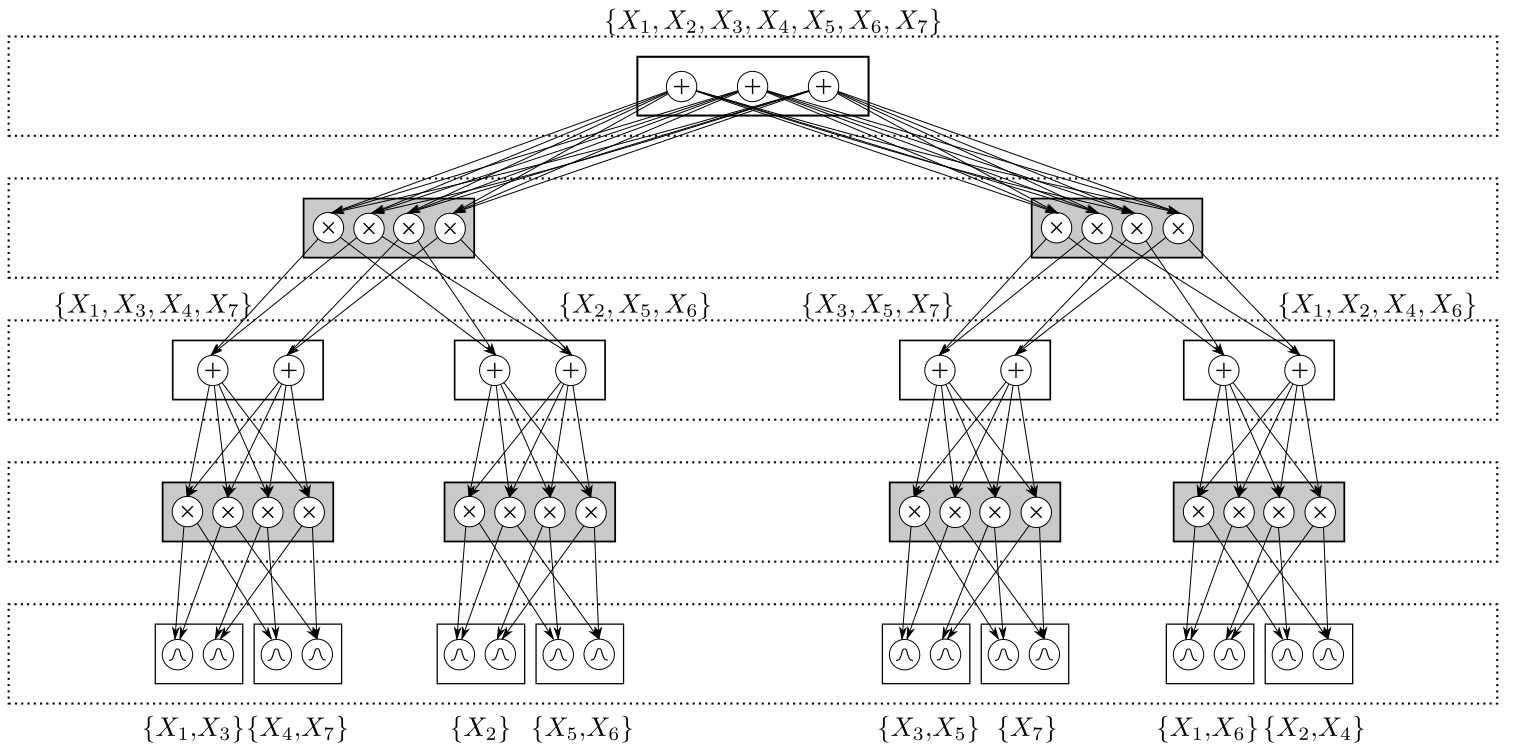
\includegraphics[scale=0.265]{Figures/RAT-SPN.png}
\end{figure}
As mentioned above, RAT-SPNs are trained in a "classical deep learning manner", i.e. employing automatic differentiation, SGD and GPU support. More specifically, let $\mathit{X} = \{(\mathbf{x}_1,\mathit{y}_1),...,(\mathbf{x}_N,\mathit{y}_N)$ be a training set of input $\mathbf{x}_n$ and class labels $\mathbf{y}_n$. Furthermore, let $\mathit{S}_C$ be the $c^{th}$ output of the RAT-SPN and $\mathbf{w}$ all SPN parameters. RAT-SPNs training is performed by minimizing the objective

\begin{equation}\label{objective}
	O(\mathbf{w}) = \lambda \mathbf{CE}(\mathbf{w}) + (1-\lambda)n\mathbf{LL}(\mathbf{w})
\end{equation}

where $\mathbf{CE}(\mathbf{w})$ is the cross-entropy

\begin{equation}\label{cross-entropy}
	\mathbf{CE}(\mathbf{w}) = -\frac{1}{\mathit{N}}\sum_{n} log\frac{\mathit{S}_{\mathit{y_n}}(\mathbf{x}_n)}{\sum_{\mathit{y'}}\mathit{S}_{\mathit{y'}}(\mathbf{x}_n)}
\end{equation}

and n$\mathbf{LL}(\mathbf{w})$ is the normalized negative log-likelihood

\begin{equation}\label{nll}
	n\mathbf{LL}(\mathbf{w}) = -\frac{1}{\mathit{N}|\mathbf{X}|}\sum_{n} log\mathit{S}_{\mathit{y_n}}.
\end{equation}
When setting $\lambda = 1$, purely cross-entropy is optimized (discriminative setting), while for $\lambda = 0$ maximum likelihood training is performed (generative setting). For $0 < \lambda < 1$, we have a continuum of hybrid objectives, trading off the generative and dsicriminative character of the model.

The size of RAT-SPN can be easily controlled via the structural parameters \textit{D}, \textit{R}, \textit{S} and \textit{I}. RAT-SPNs with many parameters, however, tend to overfit just like regular neural networks, which requires regularization. One of the classical techniques that boosted deep learning models is the well-known \textit{dropout} heuristic \cite{srivastava2014dropout}, setting inputs and/or hidden units to zero with a certain probability \textit{p}, and rescaling the remaining units by $\frac{1}{\mathit{p}}$. In RAT-SPNs two types of dropout are exploited:

\begin{enumerate}[I.]
  \item \textit{Dropout at inputs.} It essentially consists in marking input features as missing at random;
  \item \textit{Dropout at sums.} As discussed in [\cite{poon2011sum}, \cite{DBLP:journals/corr/ZhaoMP15}, \cite{DBLP:journals/corr/PeharzGPD16}], sum nodes in SPNs can be interpreted as marginalized latent variables, akin to the latent variable interpretation in mixture models. In RAT-SPNs a whole region can be interpreted as a single latent variable, and the weights of each sum node in this region as the conditional distribution of this variable. While the latent variables are not observed, the idea is to employ a simple probabilistic version of dropout, by introducing artificial observations for them. For example, if the sum nodes in a particular region have \textit{K} children (i.e. the corresponding variable \textit{Z} has \textit{K} states), then the artificial information that \textit{Z} assumes a state in some subset of $\{1,...,\mathit{K}\}$ can be introduced. By doing this for each latent variable in the network, the results essentially consists in selecting a small sub-structure of the whole SPN to explain the data. 
\end{enumerate}

\section{Abduction}
A central theme in the study of human reasoning is the construction of explanations that give us an understanding of the world we live in. Broadly speaking, abduction is a reasoning process invoked to explain a puzzling observation. A typical example is a practical competence like medical diagnosis. When a doctor observes a symptom in a patient, he hypothesizes about its possible causes, based on his knowledge of the causal relations between diseases and symptoms. This is a practical setting. Abduction also occurs in more theoretical scientific contexts. For instance, it has been claimed \cite{Peirce1932} that when Kepler discovered that Mars had an elliptical orbit, his reasoning was abductive.

Charles Sanders Peirce (1839-1914), the founder of American pragmatism was the first philosopher to give a logical form to abduction. In his early theory Peirce proposed three modes of reasoning: deduction, induction and abduction, each oh which corresponds to a syllogistic form, illustrated by the following, often quoted example \cite{Peirce1932}:
\vspace{1\baselineskip}

\textit{DEDUCTION}

Rule - All the beans from this bag are white.

Case - These beans are from this bag.

Results - These beans are white.
\vspace{1\baselineskip}

\textit{INDUCTION}

Case - These beans are from this bag.

Result - These beans are white.

Rule - All the beans from this bag are white.
\vspace{1\baselineskip}

\textit{ABDUCTION}

Rule - All the beans from this bag are white.

Results - These beans are white.

Case - These beans are from this bag.
\vspace{1\baselineskip}

Of these, deduction is the only reasoning which is completely certain, infering its 'Results' as a necessary conclusion. Induction produces a 'Rule' validated only in the 'long run' \cite{Peirce1932}, and abduction merely suggests that something may be 'the Case' \cite{Peirce1932}. The abduction is, according to Peirce, the only reasoning form that can increase our knowledge, i.e. suggest new ideas, gueess, predict. Actually, all three inference mechanisms described above allow to increase our knowledge, even if in different order and measure, but only abduction is entirely aimed at this increase. It is also true that abduction is the most subjected to error. As with induction, abduction does not contain in itself its logic validity and it has to be empirically validated; it will never be possible to have an absolute validation, but only a probabilistic one.

In the context of formal logic, abduction is often defined as follows:

\begin{definition}{\textbf{(Abduction)}}
\label{def:abduction}
Given a logical theory $\mathit{T}$ representing the expert knowledge and a formula $\mathit{Q}$ representing an observation on the problem domain, abductive inference searches for an explanation formula $\varepsilon$ such that:
\begin{itemize}
  \item $\varepsilon$ is satisfiable\footnote{If $\varepsilon$ contains free variables, $\exists(\varepsilon)$ should be satisfiable w.r.t. $\mathit{T}$.} w.r.t. T and
  \item it holds that\footnote{Or, more general, if $\mathit{Q}$ and $\varepsilon$ contain free variables: $\mathit{T} \models \forall(\varepsilon \rightarrow \mathit{Q}) $} $\mathit{T} \models \varepsilon \rightarrow \mathit{Q}$.
\end{itemize}
\end{definition}
In general, $\varepsilon$ will be subjected to further restrictions such as the aforementioned minimality criteria and criteria restricting the form of the explanation formula (e.g. by restricting the predicates that may appear in it). This view defines an abductive explanation of an observation as a formula which \textit{logically entails} the observation. However, some have argued, sometimes with good reasons, that it is more natural to view an explanation as a \textit{cause} for the observation. A well-known example is as follows: the disease paresis is caused bya latent untreated form of syphilis. The probability that latent untreated syphilis leads to paresis is only 25\%. Note that in this context, the direction of entailment and causalityare opposite: syphilis is the cause of paresis but does not entail it, while paresis entails syphilis but does not cause it. Yet a doctor can \textit{explain} paresis by the hypothesis of syphilis while paresis cannot account for an \textit{explanation}s for syphilis.

In practice, examples where causation and entailment do not correspond are rare. It turns out that in many applications of abduction in AI, the theory T describes explicit \textit{causality information}. This is notably the case in model-based diagnosis and in temporal reasoning, where theories describe effects of actions. By restricting the explanation formulas to the predicates describing primitive causes in the domain, an explanation formula which entails an observation gives a cause for the observation. Hence, for this class of theories, the logical entailment view implements the causality view on abductive inference.

In the context of logic programming, the study of abductive inference started at the end of the eighties as an outcome of different attempts to use logic programming for solving AI-problems. Facing the limitations of standard logic programming for solving these problems, different researchers proposed to extend logic programming with abduction. Eshghi \cite{Eshghi198801562579} introduced abduction in logic programming in order to solve planning problems in the Event Calculus \cite{Kowalski1989}. In this approach, abduction solves a planning goal by explaining it byan ordered sets of events -a plan- that entails the planning goal. This approach was further explored byShanahan \cite{Shanahan198901}, Missiaen et al. \cite{Eshghi198801562579},\cite{10.1093/logcom/5.5.579}, Denecker \cite{Denecker200112}, Jung \cite{SHANAHAN2000207} and recently in \cite{Kakas1998ACLPAC},\cite{KAKAS2000129}. In parallel to these studies of abduction as an inferential method, Eshghi and Kowalski \cite{Eshghi198801234235} and later Kakas and Mancarella in \cite{Kakas199001},\cite{Kakas1990OnTR} and Dung in \cite{Dung1991NegationsAH}, used abduction as a semantical device to describe the non-monotonic semantics of Logic Programming (in a wayanalogous to Poole in \cite{POOLE198827}). In \cite{Denecker2001125},\cite{10.1007/3-540-59487-6_2}, abductive logic programming was investigated from a knowledge representation point of view and its suitabilityfor representing and reasoning on incomplete information and definitional and assertional knowledge was shown. For these reasons, Abductive Logic Programming1 (ALP) \cite{10.1093/logcom/2.6.719},\cite{Kakas98therole} was recognized as a promising computational paradigm that could resolve many limitations of logic programming with respect to higher level knowledge representation and reasoning tasks. ALP has manifested itself as a framework for declarative problem solving suitable for a broad collection of problems.

\section{Classification}
\label{classification}
\textit{Classification} is a type of supervised learning that consists in building a classifier from a set of examples labeled by their classes or precedents (learning step) and then predicting the class of new examples by using the generated classifiers (classification step). More formally, let:

\begin{itemize}
  \item $\mathit{X}$ be the instance space (whose elements correspond to the observations);
  \item $\mathit{C}$ be a non-empty finite set (whose elements correspond to the classes/labels);
  \item $\mathit{c}: \mathit{X} \rightarrow \mathit{C}$ be the classification function to be learned;
  \item $\mathit{H}$ be the hypothesis space;
  \item $\mathit{h} \in \mathit{H}$ such that $h: \mathit{X} \rightarrow \mathit{C}$.
\end{itemize}
Given a sequence of training examples $\{(\mathbf{x}_1,\mathit{c}_1),...,(\mathbf{x}_n,\mathit{c}_n)\}$, where  $\mathbf{x}_i \in \mathit{X}$, $\mathit{c}_i \in \mathit{C}$ and $\mathit{c}_i = \mathit{c}(\mathbf{x}_i)$, the goal is to find $\mathit{h}$ such that $\mathit{h}(\mathbf{x}_i) = \mathit{c}(\mathbf{x}_i)$ $\forall \mathbf{x}_i \in \mathit{X}$.

In this thesis work, we are interested in a slightly different classification task, in which the known information about training examples is not directly their associated class but an aggregate information deriving from it. More formally, this task differs from the one described above in the following respects:

\begin{itemize}
  \item let $\mathit{f}: \mathit{C} \times ... \times \mathit{C} \rightarrow \mathit{F}$ be an aggregate non-injective function with arity $m$, where $\mathit{F}$ is a non-empty finite set;
  \item training examples form is $\{((\mathbf{x}_1,...,\mathbf{x}_m),\mathit{f}_1),...,((\mathbf{x}_{n-m+1},...,\mathbf{x}_n),\mathit{f}_{\frac{n}{m}})\}$, 
  where $\mathbf{x}_i \in \mathit{X}$, $\mathit{f}_i \in \mathit{F}$ and 
\begin{equation}\
	\mathit{f}_i = \mathit{f}(\mathit{c}_{m(i-1)+1},...,\mathit{c}_{m(i-1)+1+m}) = \mathit{f}(\mathit{c(\mathbf{x}_{m(i-1)+1})},...,\mathit{c(\mathbf{x}_{m(i-1)+1+m})}).
\end{equation}
\end{itemize}
Basically, training examples are grouped into tuples with cardinality $m$, on whose corresponding labels a function $\mathit{f}$ is applied. Note that:

\begin{itemize}
  \item the classifier knows how to compute $\mathit{f}$ (and this information will be encapsulated in the knowledge domain of the symbolic module); 
  \item if $\mathit{f}$ was injective, such classification task just would come back to the "standard" one, since the model would be able to deterministically derive the correct classes from the aggregate information.
\end{itemize}